\documentclass{article}
\usepackage[utf8]{inputenc}
\usepackage{tikz}
% \usetikzlibrary{arrows}
\usepackage{natbib}
\usepackage{graphicx}
\usepackage{amsmath}
\usepackage{verbatim}
\usepackage{hyperref}
\hypersetup{
    colorlinks=true,
    linkcolor=blue,
    filecolor=magenta,      
    urlcolor=cyan,
}

\usepackage{caption}
\usepackage{subcaption}
\usepackage{makecell}
\usepackage{dirtytalk}

\usepackage[a4paper, margin=0.75in]{geometry}
\usepackage{appendix}

\begin{document}


\title{Memory Bandwidth and Latency Analysis: AMD Rome, Intel Cascade Lake and Ice Lake Servers}
\author{Vamsi Sripathi\thanks{Intel Corp. - IAGS/DXPS/DEE/TCE/AWE}}
\date{September 2020}
\maketitle

\tableofcontents
\listoffigures
\listoftables
\newpage

\section{Introduction}
As Moore's law pushes the compute capabilities, it's imperative to study the bandwidth and latency characteristics of the memory sub-system in order to design a well-balanced CPU architecture. Figure-\ref{figure:1} shows one of the approaches to evaluate the memory hierarchy where each of the axis represents a control variable that impacts the observed performance, namely --
\begin{enumerate}
    \item Memory Hierarchy: Modern CPU's consists of different layers of memory pools. These include multiple levels of on-chip CPU data caches, on-chip multi-channel DRAM (MCDRAM), off-chip DDR. In addition, many CPU's support non-uniform memory access (NUMA) which acts as another memory tier.
    \item Application Threads: CPU vendors have taken different architectural routes (e.g., chiplet, large mesh) in scaling the number of cores. As the number of cores in modern CPU's increase, the cost of implementing cache coherency protocols get expensive. On these systems, the number of application threads employed and how these threads are pinned to underlying cpu cores gives an ability to understand the strengths and weaknesses of a CPU architecture.
    \item Traffic Pattern: The type of memory traffic generated play a defining role in determining the performance. After all, the memory bandwidth requirements of a dense matrix-matrix multiplication is vastly different from a stencil kernel. In addition, the cache write policies also impact performance depending upon whether a non-temporal store instruction is used in writing back the date to main memory.
\end{enumerate}

\begin{figure}
\centering
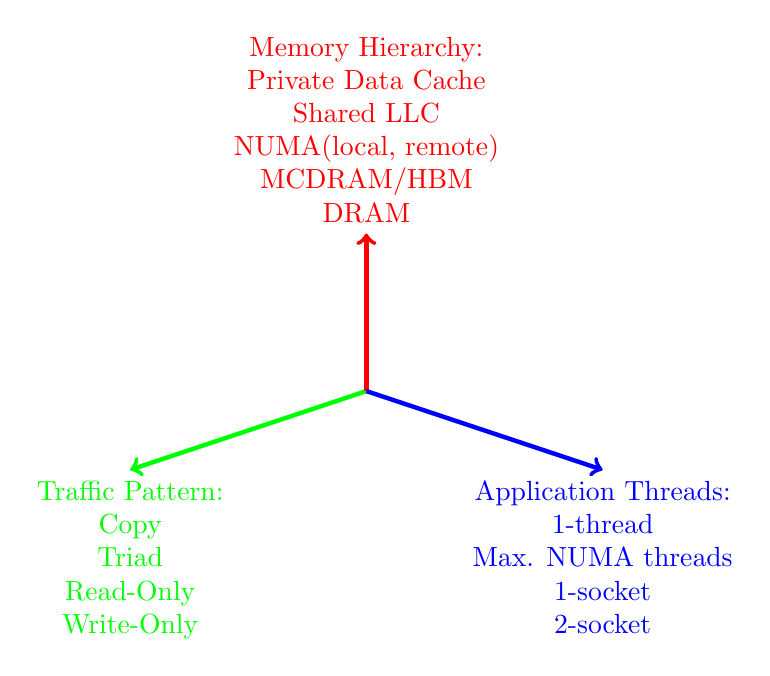
\begin{tikzpicture}
\draw[green, ultra thick, ->] (0,1) -- (-3,0)node[align=center, below] {Traffic Pattern:\\Copy\\Triad\\Read-Only\\Write-Only};
\draw[red, ultra thick, ->] (0,1) -- (0,3)node[align=center, above] {Memory Hierarchy:\\Private Data Cache\\Shared LLC\\NUMA(local, remote)\\MCDRAM/HBM\\DRAM};
\draw[blue, ultra thick, ->] (0,1) -- (3,0)node[align=center, below] {Application Threads:\\1-thread\\Max. NUMA threads\\1-socket\\2-socket};
\end{tikzpicture}
\caption{Memory sub-system study} \label{figure:1}
\end{figure}

\subsection{Scope of Study}
This report aims to characterize the memory bandwidth and latency for the following 3 CPU architectures:
\begin{enumerate}
    \item AMD Rome (2$^{nd}$ generation EPYC Processors)
    \item Intel Cascade Lake (2$^{nd}$  generation Xeon Scalable Processors)
    \item Intel Ice Lake (3$^{rd}$  generation Xeon Scalable Processors)
\end{enumerate}
Since memory bandwidth and latency is a broad topic, we will limit the scope of this study to the following aspects --
\begin{enumerate}
\item More emphasis on DDR memory bandwidth followed by cache bandwidth and latency.
\item Synthetic kernels consisting of contiguous access pattern.
\end{enumerate}

In the following sections, we will describe the experiments setup and benchmark methodology. This is followed by providing the DRAM memory bandwidth results for different traffic patterns, thread configurations, type of store instructions and NUMA domain. Next, we will provide the cache bandwidth and latency results. 

\section{Experiments Setup}
\subsection{Hardware Platforms}
The details of the CPU configuration benchmarked in this study are listed in table-\ref{table:1}. It is important to note that the CPU's have different memory channels, memory speed, number of cores etc. However, they are the top end of the SKU's for the corresponding platform and would reflect the best possible performance as observed by end users. In the rest of the document, we will refer to the CPU platforms by their corresponding code-names.

\begin{table}[h!]
\centering
 \begin{tabular}{|l|c|c|c|} \hline
& AMD Epyc 7742 & Intel Xeon 8268 & Intel ICX XCC \\\hline
Code name & Rome & Cascade Lake (CLX) & Ice Lake (ICX) \\ \hline
Number of sockets & 2 & 2 & 2 \\ \hline
Number of cores per socket & 32 & 24 & 32 \\ \hline
Total number of cores & 64 & 48 & 64 \\ \hline
LLC per socket & 256 MB & 35.7 MB & 48.3 MB \\ \hline
Total memory & 264 GB & 197 GB & 264 GB \\ \hline
Memory type & DDR4 @ 3200 MT/s & DDR4 @ 2933 MT/s & DDR4 @ 3200 MT/s \\ \hline
Memory channels per socket & 8 & 6 & 8 \\ \hline
Theoretical Peak B/W per socket & 204.8 GB/s & 140.8 GB/s & 204.8 GB/s\\   \hline
Theoretical Peak B/W & 409.6 GB/s & 281.6 GB/s & 409.6 GB/s\\   \hline
\end{tabular}
\caption{Hardware Platforms}
\label{table:1}
\end{table}

The theoretical peak memory bandwidth is calculated as: 
\begin{align*}
 Peak\: B/W\: (GB/s) = x\: GT/s\: \times\: 8 \:bytes\_per\_channel\: \times\:  n\: channels\_per\_socket \times m\: sockets
\end{align*}

\subsection{STREAM Benchmark}
STREAM is a widely used standard benchmark to characterize the memory performance. It consists of the following 4 kernels -- Copy, Scale, Add, Triad. The characteristics of these kernels are listed in table-\ref{table:2}. As can be observed from the table, Scale and Add process the same number of bytes as Copy and Triad respectively and only differ in the floating-point operations. The differences in floating-point calculations is insignificant as these operations are memory-bound. Hence, we do not show the performance of these two kernels in the remaining part of the report.

To cover additional traffic patterns, we developed two more kernels representing 100\% read (Reduce) and 100\% write traffic (Fill). The Reduce kernel performs a vector reduction by an \textit{add} opeartor and the Fill kernel writes a constant scalar value to all elements of a buffer. The source code for these kernels can be accessed at the following internal GIT repository \url{https://gitlab.devtools.intel.com/vsripath/stream/}

\subsubsection{Target ISA}
The ISA used determines how many number of bytes are transferred to/from memory from/to CPU registers in a single vector instruction. AVX2 and AVX512F vector instructions operate on 256b and 512b wide CPU registers respectively and hence transfer 32B and 64B per load/store instruction respectively. STREAM benchmark is compiled with Intel C Compiler with the relevant flags to generate the optimal instruction generation for the target processor. The highest ISA supported on AMD Rome and Intel CLX, ICX is AVX2 and AVX512F respectively. Hence, AVX2 and AVX512F instructions are generated in the binary that is executed on AMD Rome and Intel CLX, ICX respectively. Refer to the makefile at the aforementioned GIT source repository for all the Compiler flags used in building the binaries used in this study.

\subsubsection{Cache Write Policy: vmovpd vs vmovntpd}
A CPU caches' write policy determines how and when the data in cache is written back to main memory. Usually, there are two write policies -- \textit{write-through and write-back}. Both AMD Rome and Intel CLX, ICX use \textit{write-back (WB)} cache policy. In WB policy, when the CPU modifies data, it's only updated in the cache and the write to the main memory is postponed until the cache line containing the updated data is evicted. Hence, a read-miss on a WB cache may require two memory accesses -- if modified, write the contents of the to-be evicted cache line to main memory and then fetch the requested data from main memory. For write-misses, they can be two approaches -- \textit{write-allocate, no-write allocate}. In \textit{write-allocate} policy, a store that misses the cache first fetches the cache line containing the data from main memory. And then when combined with the \textit{write-back} policy, results in an additional memory access to write the updated data back to main memory.

If we look at the STREAM kernels, we observe the following two characteristics --
\begin{itemize}
\item Full Cache Line update: There are no partial cache line modifications done by the kernels.
\item Non-Temporal Locality: The data that is written is never accessed/read again. Hence, there is no need to keep the data in cache.
\end{itemize}

Considering these aspects of STREAM kernels, we can observe that the \textit{write-allocate} policy introduces an unnecessary overhead of fetching the data to cache. This introduces additional constrains on memory bandwidth when all the cores are actively writing data to main memory. To alleviate this, we can use an alternative store instruction called \textit{non-temporal} store (vmovntpd) which by-passes the cache and directly writes to main memory.

In order to understand the impact of type of store instruction on memory bandwidth performance, STREAM benchmark is compiled in the following two configurations --
\begin{itemize}
\item Regular Stores: This configuration uses regular stores (vmovpd) that generates two memory accesses on a write-miss. We will refer to this configuration as Read-For-Ownership (RFO) in the rest of the report. RFO is a cache coherency operation specifying a read operation with intent to write to that memory address.
\item Non-Temporal (NT) Stores: This configuration uses the aforementioned vmovntpd instruction to write back directly to main memory without bringing the data into cache. We will refer to this configuration as NT in the rest of the report.
\end{itemize}

\begin{table}[h!]
\centering
 \begin{tabular}{|l|l|c|c|c|c|}
 \hline
 Kernel & Op & \makecell{Bytes Read \\ (RFO)} & \makecell{Bytes Read \\ (NT)} & Bytes Written & FLOPs \\ \hline
 COPY & \(a[i] = b[i]\)& 16 & 8 & 8 & 0\\ \hline
 SCALE & \(a[i] = scalar \times b[i]\) & 16 & 8 & 8 & 1\\ \hline
 ADD & \(c[i] = a[i] + b[i]\) & 24 & 16 & 8 & 1\\ \hline
 TRIAD & \(c[i] = a[i] + scalar \times b[i]\) & 24 & 16 & 8 & 2 \\ \hline
 REDUCE & \(sum += a[i]\) & 8 & 8 & 0 & 1 \\ \hline
 FILL & \(a[i] = constant\) & 8 & 0 & 8 & 0 \\  \hline
\end{tabular}
\caption{STREAM Kernels}
\label{table:2}
\end{table}

\subsection{Intel Memory Latency Checker}For cache bandwidth and latency analysis, we rely on the more versatile Intel Memory Latency Checker.


\subsection{Runtime Settings}
Table-\ref{table:3} shows the run-time settings used for most of the results presented in this study. Where we depart from these settings, we will explicitly call out the changes in the corresponding section.

\begin{table}[h!]
\centering
\begin{tabular}{|c|c|c|c|}  \hline
 & AMD Rome 7742 & Intel Xeon 8268 & Intel ICX XCC \\ \hline
NUMA per socket & 4 & 1 & 1 \\ \hline
Operating System & \multicolumn{3}{c|}{CentOS Linux 7 (Core)} \\  \hline
Kernel & \multicolumn{3}{c|}{3.10.0-1127.18.2.el7.crt1.x86\_64} \\ \hline
CPU Turbo Boost & \multicolumn{3}{c|}{Enabled} \\  \hline
CPU Scaling Governor & \multicolumn{3}{c|}{userspace} \\  \hline
CPU Scaling Driver & \multicolumn{3}{c|}{acpi-cpufreq} \\  \hline
Transparent Huge Pages & \multicolumn{3}{c|}{Enabled} \\  \hline
Intel C Compiler & \multicolumn{3}{c|}{ICC 19.1.2.254 20200623} \\  \hline
Hyper-Threading & \multicolumn{3}{c|}{\makecell{Enabled in HW,\\but logical threads are not used in benchmarking}} \\
\hline
OpenMP Thread Affinity & \multicolumn{3}{c|}{KMP\_AFFINITY = \say{granularity=fine,compact,1,0}} \\ \hline
\end{tabular}
\caption{Runtime Settings}
\label{table:3}
\end{table}

\section{DRAM Bandwidth}
In the following sub-sections, we will look at the peak achieved memory bandwidth by different CPU's in 1-core, 1-socket and 2-socket configuration. We will also evaluate the scaling performance within a socket and the impact of NUMA domains and OpenMP thread to CPU core affinity as well. Each sub-section contains performance data to primarily answer the following two questions -- 

\begin{enumerate}
\item How does the different CPU architectures compare against each other?
\item What is the impact of using RFO and NT stores on a given architecture?
\end{enumerate}

\subsection{1-Core}

\begin{figure}[!hb]
    \centering
    \begin{subfigure}[!hb]{0.3\textwidth}
         \centering
         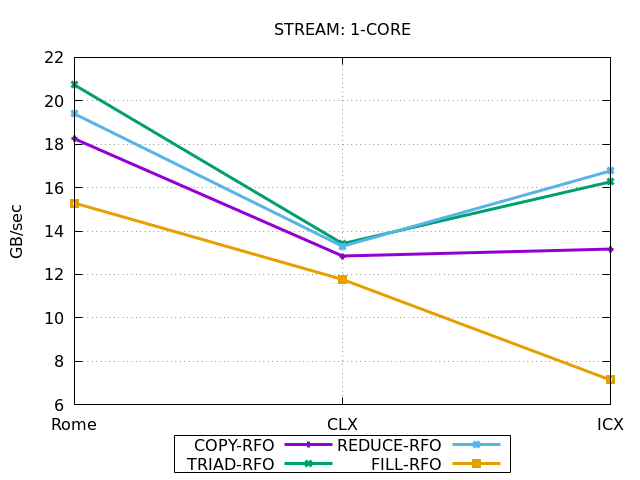
\includegraphics[width=\textwidth]{../mem_bw_core/mb_core_rfo}
         \caption{RFO}
         \label{figure:mem_bw_core_rfo}
    \end{subfigure}
    \begin{subfigure}[!hb]{0.3\textwidth}
         \centering
         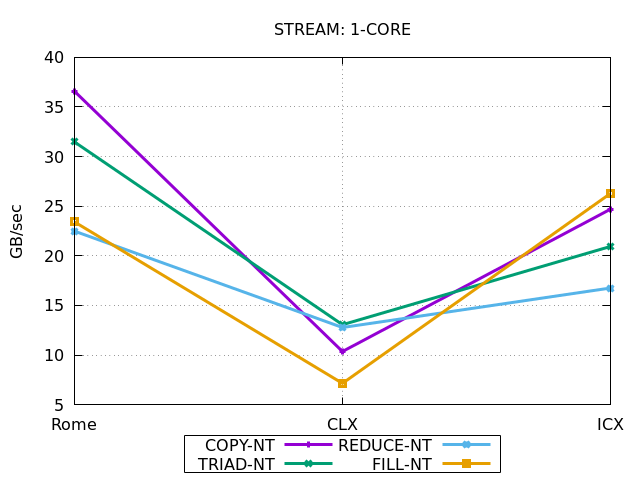
\includegraphics[width=\textwidth]{../mem_bw_core/mb_core_nt}
         \caption{NT}
         \label{figure:mem_bw_core_nt}
    \end{subfigure}
    \begin{subfigure}[!hb]{0.3\textwidth}
         \centering
         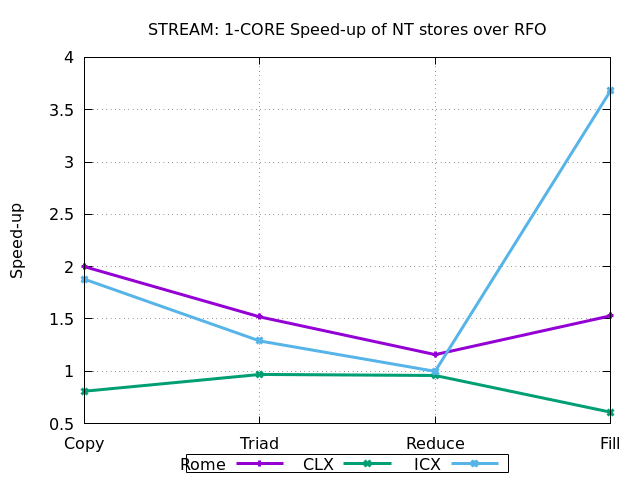
\includegraphics[width=\textwidth]{../mem_bw_core/mb_core_nt_rfo}
         \caption{Speed-up of NT over RFO}
         \label{figure:mem_bw_core_nt_rfo}
    \end{subfigure}

    \caption{STREAM 1-core DRAM bandwidth}
    \label{figure:mem_bw_core}
\end{figure}

\subsubsection{Peak Bandwidth with RFO}
Figure-\ref{figure:mem_bw_core_rfo} RFO observations:
\begin{enumerate}
\item Rome vs ICX: Even though these two processors have identical DRAM configuration, Rome delivers higher bandwidth across the kernels. 
\item ICX vs CLX: Comparing gen-to-gen Xeon performance, there is a slow-down of 37\% and 52\% for Reduce and Fill kernels respectively on ICX. This is despite the fact that ICX has higher DDR4 memory speed and channels.
\item Table-\ref{table:mem_bw_core_rfo} summarizes the speed-up of all kernels.
\end{enumerate}

\begin{table}[h!]
\centering
\begin{tabular}{|c|c|c|c|c|c|c|}  \hline
Kernel&Rome&CLX&ICX & ICX/Rome & CLX/Rome & ICX/CLX \\ \hline 
Copy & 18.25 & 12.85 & 13.17  & 0.72 & 0.70 & 1.02 \\ \hline 
Triad & 20.73 & 13.42 & 16.27  & 0.78 & 0.65 & 1.21 \\ \hline 
Reduce & 19.40 & 13.30 & 16.77  & 0.86 & 0.69 & 1.26 \\ \hline 
Fill & 15.29 & 11.77 & 7.14  & 0.47 & 0.77 & 0.61 \\ \hline 
\end{tabular}

% Kernel & Rome/ICX & Rome/CLX & ICX/CLX \\ \hline
% Copy & 1.51x & 1.49x & 0.99x \\ \hline
% Triad & 1.73x & 1.71x & 0.99x \\ \hline
% Reduce & 2.26x & 1.65x & 0.73x \\ \hline
% Fill & 1.97x & 1.30x & 0.66x \\ \hline
\caption{1-core peak bandwdith: RFO}
\label{table:mem_bw_core_rfo}
\end{table}

\subsubsection{Peak Bandwidth with NT}

Figure-\ref{figure:mem_bw_core_nt} NT observations:
\begin{enumerate}
\item Rome vs ICX: Similar to the trend observed with RFO stores, Rome delivers higher bandwidth across the kernels with the speed-up over ICX even greater. 
\item ICX vs CLX: On ICX, the Fill kernel using NT stores shows marked improved over CLX. And the rest of the kernels exhibit slow-down.
\item Table-\ref{table:mem_bw_core_nt} summarizes the speed-up of all kernels.
\end{enumerate}


\begin{table}[h!]
\centering
\begin{tabular}{|c|c|c|c|c|c|c|}  \hline
Kernel&Rome&CLX&ICX & ICX/Rome & CLX/Rome & ICX/CLX \\ \hline 
Copy & 36.59 & 10.36 & 24.70  & 0.68 & 0.28 & 2.38 \\ \hline 
Triad & 31.48 & 13.06 & 20.95  & 0.67 & 0.41 & 1.60 \\ \hline 
Reduce & 22.49 & 12.78 & 16.76  & 0.75 & 0.57 & 1.31 \\ \hline 
Fill & 23.42 & 7.15 & 26.29  & 1.12 & 0.31 & 3.68 \\ \hline 
\end{tabular}

% Kernel & Rome/ICX & Rome/CLX & ICX/CLX \\ \hline
% Copy & 3.84x & 3.46x & 0.90x \\ \hline
% Triad & 2.69x & 1.99x & 0.74x \\ \hline
% Reduce & 2.24x & 1.72x & 0.77x \\ \hline
% Fill & 1.53x & 3.23x & 2.11x \\ \hline
\caption{1-core peak bandwdith: NT}
\label{table:mem_bw_core_nt}
\end{table}

\subsubsection{RFO vs. NT Stores}
For the different STREAM kernels, we can come up with the following expected speed-up of NT over RFO --
\begin{itemize}
\item Copy: The Copy kernel has a total of 2 (1 read, 1 write) and 3 (2-reads, 1 write) memory-ops when using NT and regular stores respectively. Hence, the ideal speed-up of NT over RFO should be 1.5x.
\item Triad: The Triad kernel has a total of 3 (2 reads, 1 write) and 4 (3 reads, 1 write) memory-ops when using NT and regular stores. Hence, the ideal speed-up of NT over RFO should be 1.33x.
\item Reduce: The Reduce kernel has 0 write ops and so the performance should remain the same with both NT and regular stores.
\item Fill: The Fill kernel has only memory write ops and so the ideal speed-up of NT over RFO should be 2x.
\end{itemize}


Figure-\ref{figure:mem_bw_core_nt_rfo} observations:
\begin{enumerate}
\item Across the CPU's, the Reduce kernel performance remains identical between NT and RFO configurations since it has no writes to main memory.
\item Rome: As can be expected, NT stores show higher performance than using regular stores which generate RFO requests. Interestingly, the speed-up of Copy kernel with NT stores exceeds the expected speed-up.
\item CLX: None of the kernels shows gains with NT. This indicates that memory bandwidth is not the constraint when using 1 core because RFO generates more memory traffic than NT. This leads to the observation that when the system is not memory bandwidth constrained (as is the case here with 1-thread), the latency of NT stores is greater than regular stores. This could be due to the fact that the hardware prefetchers do a good job of fetching the write-miss requests with regular stores. In contrast, with NT stores the hardware prefetchers have no active role since the data is never to be brought into cache.
\item ICX: Only the Fill kernel using NT stores shows higher performance than regular stores. Find out why?
\end{enumerate}


\subsection{1-Socket}
\begin{figure}[!ht]
    \centering
    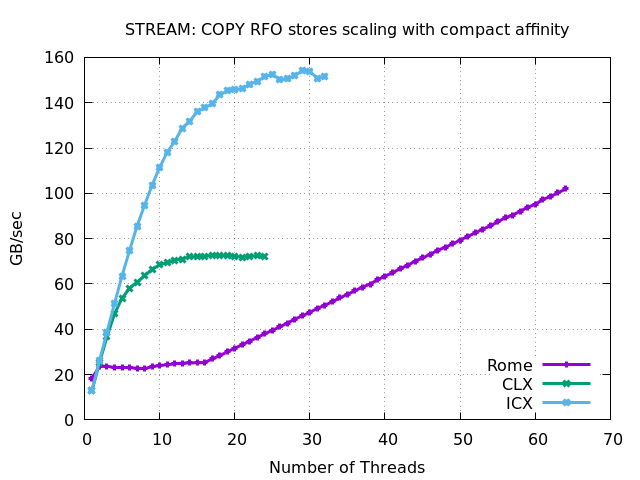
\includegraphics[width=0.45\textwidth]{../mem_bw_scale/mb_scale_compact_Copy_rfo}
    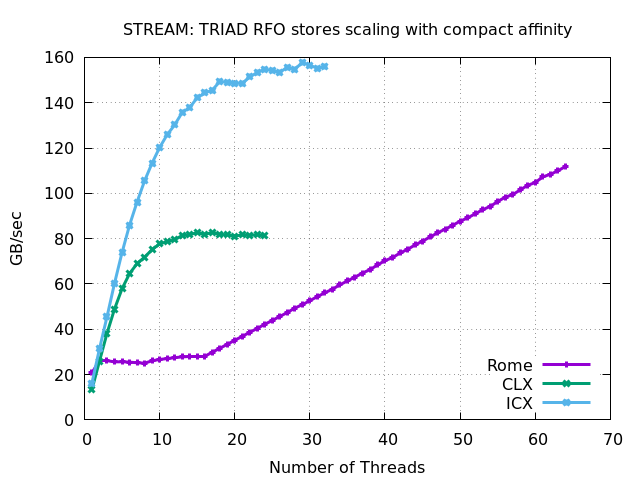
\includegraphics[width=0.45\textwidth]{../mem_bw_scale/mb_scale_compact_Triad_rfo}
    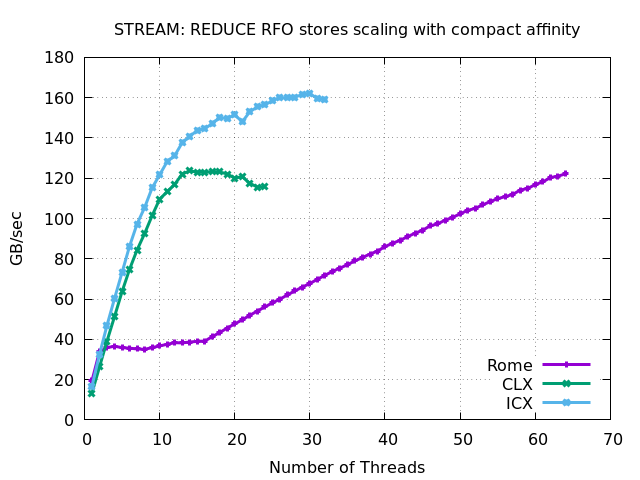
\includegraphics[width=0.45\textwidth]{../mem_bw_scale/mb_scale_compact_Reduce_rfo}
    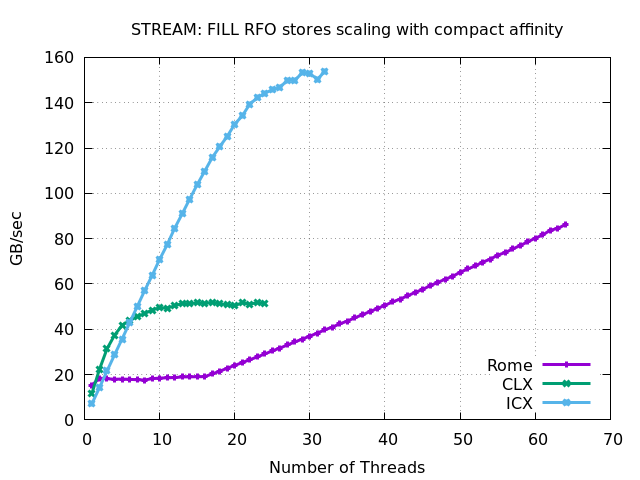
\includegraphics[width=0.45\textwidth]{../mem_bw_scale/mb_scale_compact_Fill_rfo}
    \caption{STREAM 1-socket DRAM bandwidth scaling with RFO and Compact pinning}
    \label{figure:mem_bw_scale_compact_rfo}
\end{figure}

For these experiments, Rome is configured to be in 4 NUMA domains Per Socket (NPS) mode whereas ICX and CLX are configured to have 1 NPS. Also, OpenMP threads are pinned to cores that are closer first i.e., compact mode. We will explore the performance impact of distributed pinning in the next section.

\subsubsection{Peak Bandwidth and Scaling with RFO}
Figure-\ref{figure:mem_bw_scale_compact_rfo} observations:
\begin{itemize}
\item Peak Bandwidth: Using all the cores in the socket
\begin{itemize}
\item Rome vs ICX: Contrary to 1-core performance, ICX beats Rome for all kernels using RFO stores.
\item Rome vs CLX: Rome delivers superior performance for all kernels.
\item ICX vs CLX: Comparing gen-to-gen Xeon performance, ICX delivers significant performance improvements over CLX for all kernels.
\item Table-\ref{table:mem_bw_socket_rfo} shows the speed-up of all kernels.
\end{itemize}
\item Scaling Performance: 
\begin{itemize}
\item Rome: Across the 4 kernels, Rome exhibits similar scaling performance pattern. Since Rome contains 64 cores per socket partitioned into 4 NUMA domains, each NUMA domain contains 16 cores. The data in the figure shows that the performance remains similar from 1 to 16 threads i.e., when threads are populated in NUMA domain-0. After that, the performance increases linearly with thread count and the gains from 16 to 64 threads show ideal scaling behavior.
\item CLX, ICX: In contrast to Rome, both CLX and ICX reach close to peak bandwidth using much less number of threads. In addition, CLX shows higher performance at some thread counts for Reduce and Fill kernels. 
\end{itemize}
\end{itemize}

\begin{table}[h!]
\centering
\begin{tabular}{|c|c|c|c|c|c|c|}  \hline
Kernel&Rome&CLX&ICX & ICX/Rome & CLX/Rome & ICX/CLX \\ \hline 
Copy & 101.91 & 71.92 & 151.72  & 1.49 & 0.71 & 2.11 \\ \hline 
Triad & 111.82 & 81.35 & 155.98  & 1.39 & 0.73 & 1.92 \\ \hline 
Reduce & 122.14 & 115.73 & 159.14  & 1.30 & 0.95 & 1.38 \\ \hline 
Fill & 86.25 & 51.38 & 153.83  & 1.78 & 0.60 & 2.99 \\ \hline 
\end{tabular}

% Kernel & ICX/Rome & ICX/CLX & CLX/Rome\\ \hline
% Copy & 1.40x & 2.03x & 0.69x \\ \hline
% Triad & 1.36x & 1.87x & 0.72x \\ \hline
% Reduce & 1.31x & 1.40x & 0.94x \\ \hline
% Fill & 1.76x & 2.82x & 0.62x \\ \hline
\caption{1-socket peak bandwdith: RFO}
\label{table:mem_bw_socket_rfo}
\end{table}

\subsubsection{Peak Bandwidth and Scaling with NT}

\begin{figure}[!ht]
    \centering
    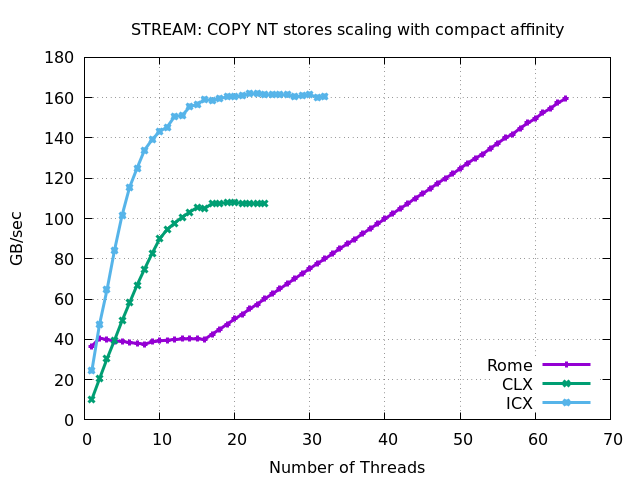
\includegraphics[width=0.45\textwidth]{../mem_bw_scale/mb_scale_compact_Copy_nt}
    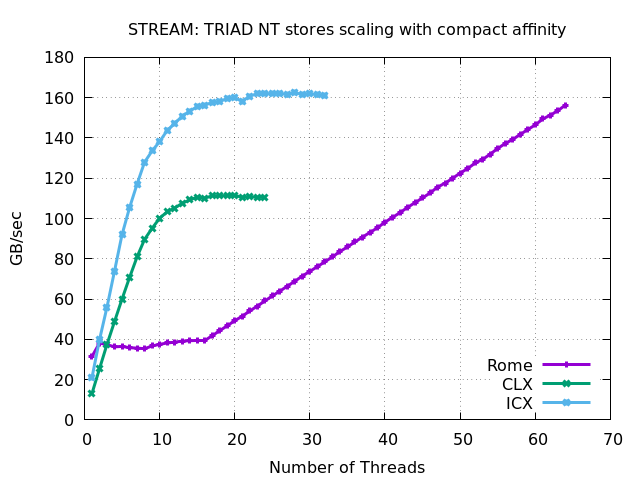
\includegraphics[width=0.45\textwidth]{../mem_bw_scale/mb_scale_compact_Triad_nt}
    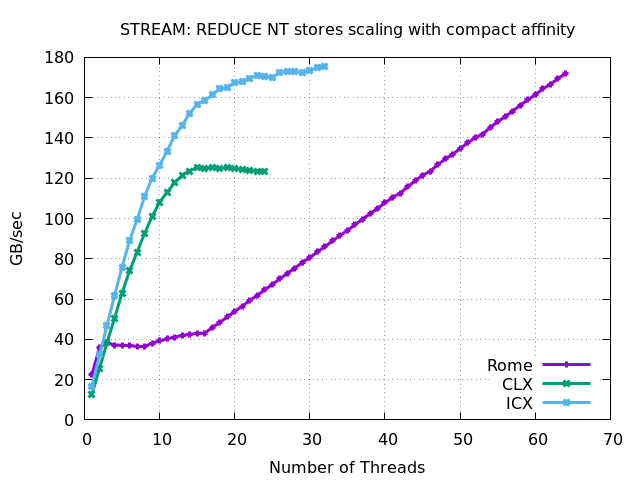
\includegraphics[width=0.45\textwidth]{../mem_bw_scale/mb_scale_compact_Reduce_nt}
    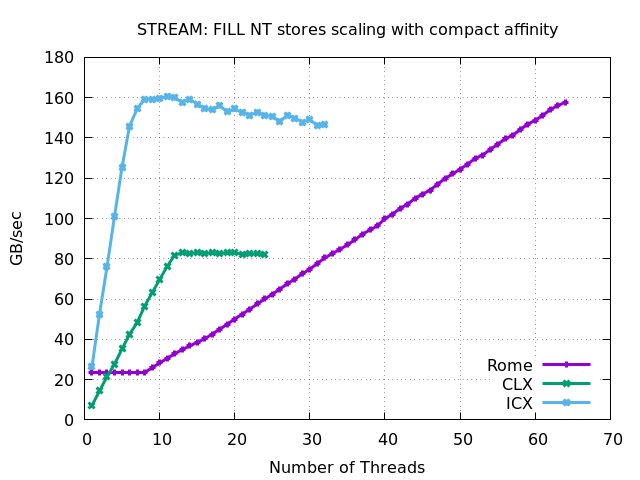
\includegraphics[width=0.45\textwidth]{../mem_bw_scale/mb_scale_compact_Fill_nt}
    \caption{STREAM 1-socket DRAM bandwidth scaling with NT Stores and Compact pinning}
    \label{figure:mem_bw_scale_compact_nt}
\end{figure}

Figure-\ref{figure:mem_bw_scale_compact_nt} observations:
\begin{itemize}
\item Peak Bandwidth: Using all the cores in the socket
\begin{itemize}
\item Rome vs ICX: Contrary to RFO, ICX delivers similar performance as Rome, with Triad showing 27\% gains and Fill showing slow-down.
\item Rome vs CLX: Rome delivers superior performance for all kernels.
\item ICX vs CLX: Comparing gen-to-gen Xeon performance, ICX delivers 40-70\% performance improvements over CLX for all kernels.
\item Table-\ref{table:mem_bw_socket_nt} shows the speed-up of all kernels.
\end{itemize}
\item Scaling Performance: The scaling profile looks similar to RFO except for the following exceptions --
\begin{itemize}
\item Rome: The Fill kernel shows gains with thread count starting at 8 instead of 16 as observed with RFO stores.
\item ICX: The Fill kernel loses performance when using all the threads in the socket. This results in reduction of about 15\% peak bandwidth for this kernel.
\end{itemize}
\end{itemize}

\begin{table}[h!]
\centering
\begin{tabular}{|c|c|c|c|c|c|c|}  \hline
Kernel&Rome&CLX&ICX & ICX/Rome & CLX/Rome & ICX/CLX \\ \hline 
Copy & 159.39 & 107.55 & 160.40  & 1.01 & 0.67 & 1.49 \\ \hline 
Triad & 156.29 & 110.45 & 161.14  & 1.03 & 0.71 & 1.46 \\ \hline 
Reduce & 171.97 & 123.45 & 175.31  & 1.02 & 0.72 & 1.42 \\ \hline 
Fill & 157.72 & 81.99 & 146.77  & 0.93 & 0.52 & 1.79 \\ \hline 
\end{tabular}

% Kernel & ICX/Rome & ICX/CLX & CLX/Rome \\ \hline
% Copy & 0.99x & 1.45x & 0.68x \\ \hline
% Triad & 1.27x & 1.44x & 0.88x \\ \hline
% Reduce & 0.99x & 1.39x & 0.71x \\ \hline
% Fill & 0.89x & 1.71x & 0.52x \\ \hline
\caption{1-socket peak bandwdith: NT}
\label{table:mem_bw_socket_nt}
\end{table}


\subsubsection{RFO vs. NT Stores}

\begin{figure}[!ht]
    \centering
    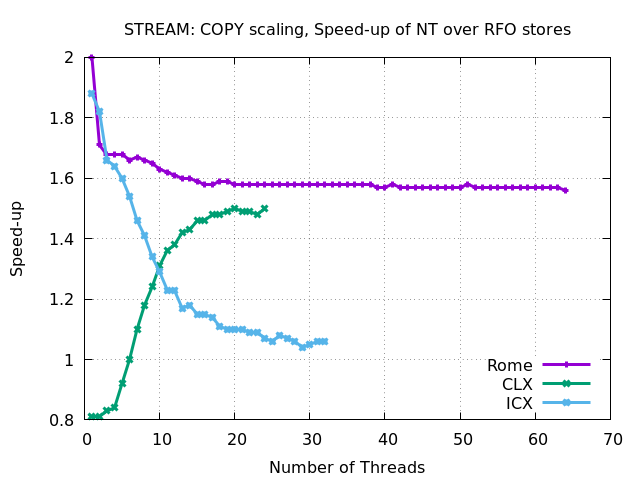
\includegraphics[width=0.45\textwidth]{../mem_bw_scale/mb_scale_compact_Copy_nt_rfo}
    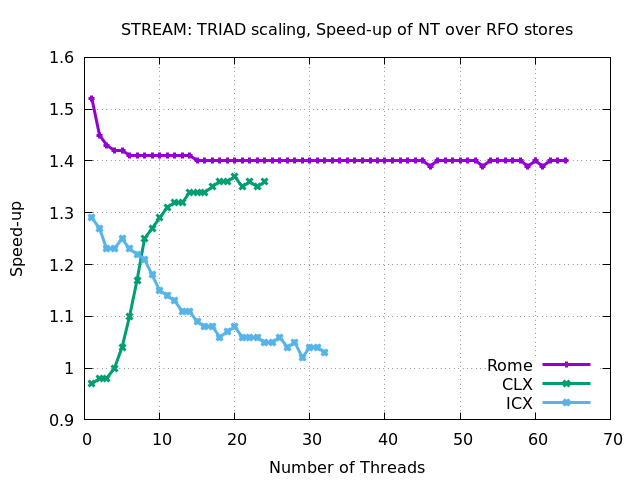
\includegraphics[width=0.45\textwidth]{../mem_bw_scale/mb_scale_compact_Triad_nt_rfo}
    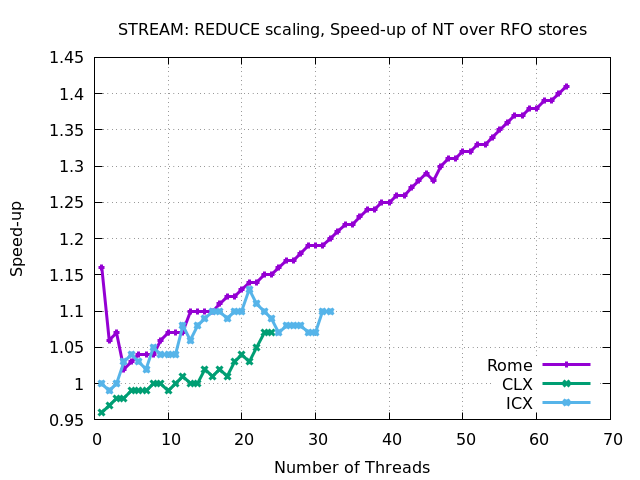
\includegraphics[width=0.45\textwidth]{../mem_bw_scale/mb_scale_compact_Reduce_nt_rfo}
    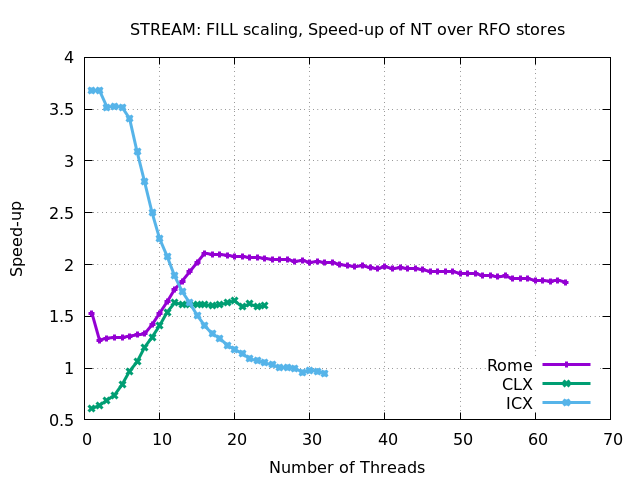
\includegraphics[width=0.45\textwidth]{../mem_bw_scale/mb_scale_compact_Fill_nt_rfo}
    \caption{STREAM 1-socket DRAM bandwidth scaling, speed-up of NT over RFO Stores}
    \label{figure:mem_bw_scale_compact_nt_rfo}
\end{figure}

\begin{enumerate}
\item Copy: As mentioned in the previous section, the ideal speed-up of NT over RFO for Copy kernel should be 1.5x. Rome matches with the expected ideal speed-up. CLX reaches the 1.5x speed-up at higher thread count whereas ICX shows far lesser gains with NT stores. Also, to be noted is that both CLX and ICX shows performance degradation with NT stores with lower thread counts which isn't the case with Rome.
\item Triad: The ideal speed-up of NT over RFO for Triad should be 1.33x. Rome reaches the ideal speed-up at some thread counts and then appears to exhibit lower gains. CLX shows expected gains at higher thread counts, whereas ICX shows maximum gains of about 10\% with NT stores. Similar to the Copy kernel, both CLX and ICX exhibit performance degradation with NT stores at lower thread counts.
\item Reduce: The performance of Reduce kernel should remain identical with both NT and regular stores. However, the Reduce kernel on Rome shows upto 40\% performance gains with NT stores. Deeper investigation of this kernel code generation revealed that the Intel compiler does aggressive unrolling when using regular stores. This results in more in-flight loads and appears to be the root-cause for the slowdown with regular stores. Interestingly, even though the Intel Compiler does the same aggressive unrolling with regular stores on CLX and ICX, these two architectures seems to be more resilient to additional in-flight loads and do not result in lower performance.
\item Fill: The ideal speed-up of NT over RFO should be 2x. Rome reaches the expected gains once the thread count is greater than the number of cores of NUMA domain. CLX and ICX exhibit different behavior for this kernel with ICX showing significant performance loss as thread count increases.
\end{enumerate}


\subsubsection{Compact vs Distributed Pinning}
The experiments with thread affinity settings make for an interesting performance study only when there are multiple NUMA domains in a socket. Since only Rome is configured to have 4 NUMA domains per socket in our setup, we will limit these experiments to Rome architecture. As mentioned earlier, Compact pinning refers to thread affinity scheme where OpenMP threads are pinned to cores that are closer to each other. In distributed pinning scheme, we affinitize the OpenMP threads to spread across the NUMA domains first. For e.g, with 4 threads this translates to using a single core on each of the 4 NUMA domains in a socket.

\begin{figure}[!ht]
    \centering
    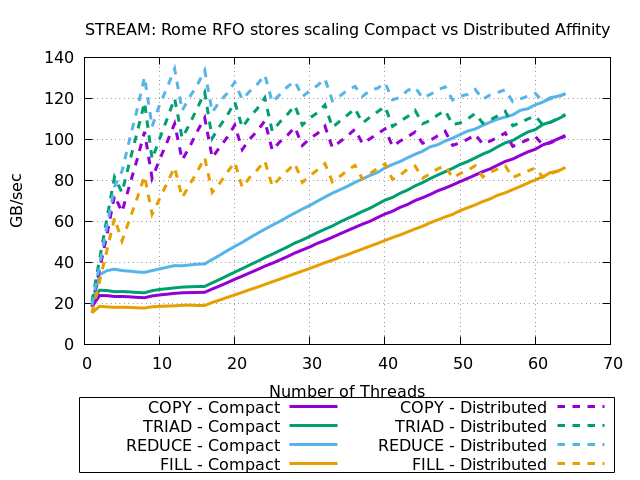
\includegraphics[width=0.45\textwidth]{../mem_bw_scale/Rome_scale_affinity_rfo}
    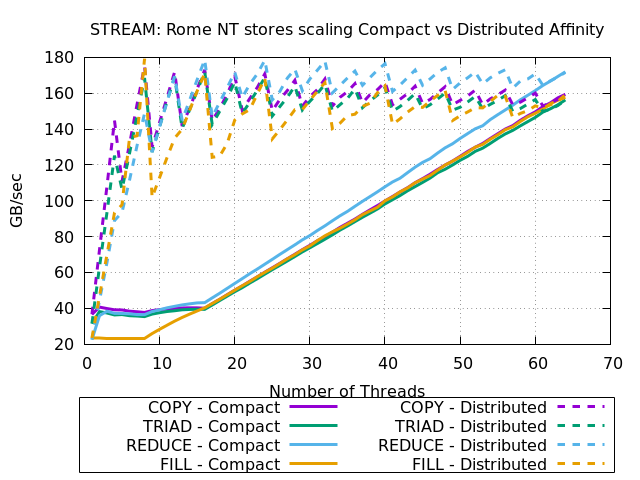
\includegraphics[width=0.45\textwidth]{../mem_bw_scale/Rome_scale_affinity_nt}
    \caption{STREAM 1-socket DRAM bandwidth: Compact vs Distributed Pinning}
    \label{figure:mem_bw_scale_affinity_rfo_nt}
\end{figure}

Figure-\ref{figure:mem_bw_scale_affinity_rfo_nt} observations:
\begin{itemize}
\item For both RFO and NT, close to peak bandwidth is achieved with fewer threads in distributed pinning when compared to compact mode.
\item RFO: The Reduce kernel with distributed affinity reaches peak bandwidth at fewer threads and then loses performance when using all the cores in the socket.
\item NT: When compared to the rest of the kernels, the Fill kernel in distributed pinning shows much less achieved bandwidth. Once the number of threads reaches more than 32, the performance is only marginally better than compact pinning.
\end{itemize}

\subsection{2-Socket}
\begin{figure}[!ht]
    \centering
    \begin{subfigure}[!hb]{0.3\textwidth}
         \centering
         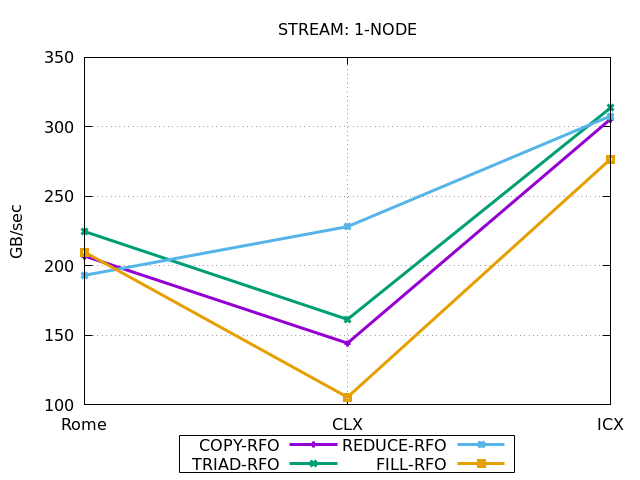
\includegraphics[width=\textwidth]{../mem_bw_node/mb_node_rfo}
         \caption{RFO}
         \label{figure:mem_bw_node_rfo}
    \end{subfigure}
    \begin{subfigure}[!hb]{0.3\textwidth}
         \centering
         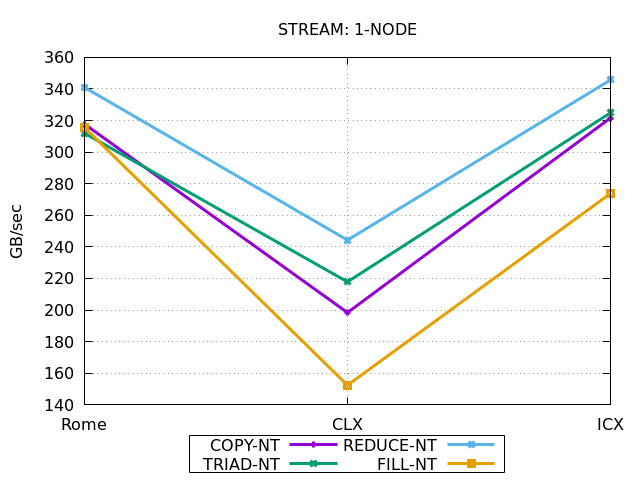
\includegraphics[width=\textwidth]{../mem_bw_node/mb_node_nt}
         \caption{NT}
         \label{figure:mem_bw_node_nt}
    \end{subfigure}
    \begin{subfigure}[!hb]{0.3\textwidth}
         \centering
         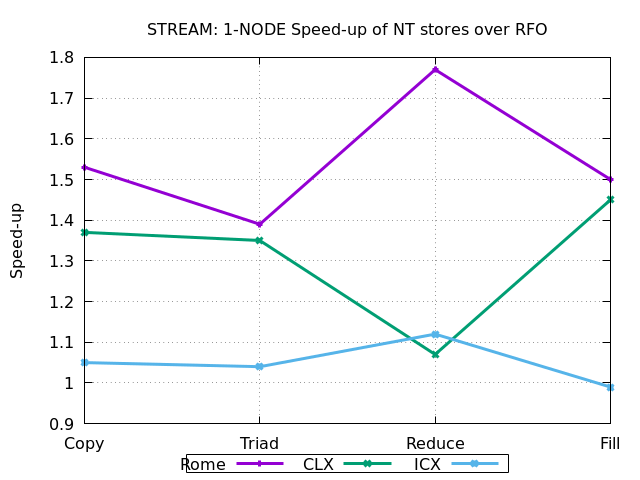
\includegraphics[width=\textwidth]{../mem_bw_node/mb_node_nt_rfo}
         \caption{Speed-up of NT over RFO}
         \label{figure:mem_bw_node_nt_rfo}
    \end{subfigure}

    \caption{STREAM 2-socket DRAM bandwidth}
    \label{figure:mem_bw_node}
\end{figure}


Since each socket has it's own set of memory controllers, DRAM bandwidth for 2-socket scales by a factor of 2 compared to 1-socket performance. There are no unique observations when it comes to 2-socket dataand all the points made in the 1-socket section are valid here as well.
\subsubsection{Peak Bandwidth with RFO}
Figure-\ref{figure:mem_bw_node} shows the peak achieved bandwidth when all cores in a 2 socket system are accessing data to/from DRAM. Table-\ref{table:mem_bw_node_rfo}, \ref{table:mem_bw_node_nt} show the corresponding speed-up for each of the architecture with RFO and NT stores respectively..

\begin{table}[h!]
\centering
\begin{tabular}{|c|c|c|c|c|c|c|}  \hline
Kernel&Rome&CLX&ICX & ICX/Rome & CLX/Rome & ICX/CLX \\ \hline 
Copy & 207.04 & 144.30 & 305.52  & 1.48 & 0.70 & 2.12 \\ \hline 
Triad & 224.69 & 161.42 & 313.66  & 1.40 & 0.72 & 1.94 \\ \hline 
Reduce & 193.15 & 228.17 & 307.77  & 1.59 & 1.18 & 1.35 \\ \hline 
Fill & 209.83 & 105.40 & 276.74  & 1.32 & 0.50 & 2.63 \\ \hline 
\end{tabular}

% \begin{tabular}{|c|c|c|c|} \hline
% Kernel & ICX/Rome & ICX/CLX & CLX/Rome\\ \hline
% Copy & 1.34x & 2.04x & 0.66x \\ \hline
% Triad & 1.36x & 1.87x & 0.72x \\ \hline
% Reduce & 1.57x & 1.34x & 1.17x \\ \hline
% Fill & 1.49x & 2.61x & 0.57x \\ \hline
\caption{2-socket peak bandwdith: RFO}
\label{table:mem_bw_node_rfo}
\end{table}


\subsubsection{Peak Bandwidth with NT}
Figure-\ref{figure:mem_bw_node} shows the peak achieved bandwidth using NT stores.
\begin{table}[h!]
\centering
\begin{tabular}{|c|c|c|c|c|c|c|}  \hline
Kernel&Rome&CLX&ICX & ICX/Rome & CLX/Rome & ICX/CLX \\ \hline 
Copy & 317.77 & 198.35 & 321.62  & 1.01 & 0.62 & 1.62 \\ \hline 
Triad & 311.98 & 217.81 & 324.89  & 1.04 & 0.70 & 1.49 \\ \hline 
Reduce & 341.00 & 244.26 & 345.71  & 1.01 & 0.72 & 1.42 \\ \hline 
Fill & 315.62 & 152.32 & 273.78  & 0.87 & 0.48 & 1.80 \\ \hline 
\end{tabular}

% \begin{tabular}{|c|c|c|c|} \hline
% Kernel & ICX/Rome & ICX/CLX & CLX/Rome \\ \hline
% Copy & 0.99x & 1.51x & 0.66x \\ \hline
% Triad & 1.26x & 1.43x & 0.88x \\ \hline
% Reduce & 0.99x & 1.38x & 0.72x \\ \hline
% Fill & 0.82x & 1.67x & 0.49x \\ \hline
\caption{2-socket peak bandwdith: NT}
\label{table:mem_bw_node_nt}
\end{table}



\subsection{NUMA}
\subsubsection{1-Core, 1-Socket: RFO}
\begin{figure}[!ht]
    \centering
    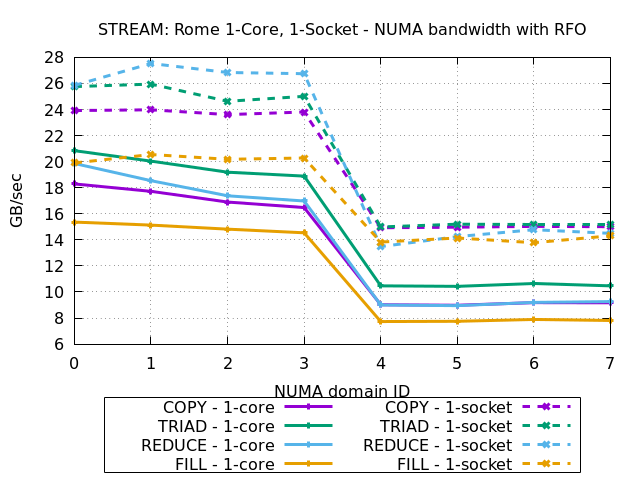
\includegraphics[width=0.3\textwidth]{../mem_bw_numa/Rome_numa_nps4_compact_rfo}
    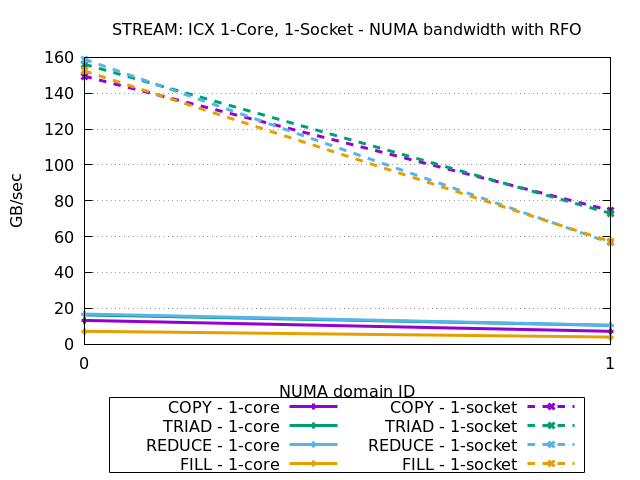
\includegraphics[width=0.3\textwidth]{../mem_bw_numa/ICX_numa_nps1_compact_rfo}
    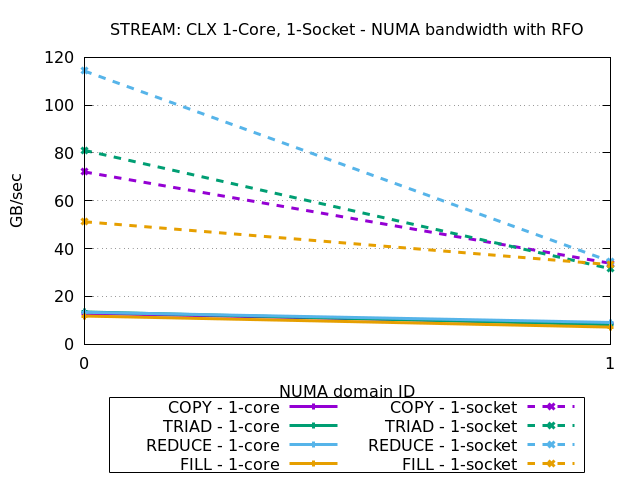
\includegraphics[width=0.3\textwidth]{../mem_bw_numa/CLX_numa_nps1_compact_rfo}
    \caption{STREAM 1-Core, 1-socket NUMA bandwidth with RFO}
    \label{figure:mem_bw_numa_rfo}
\end{figure}

\subsubsection{1-Core, 1-Socket: NT}
\begin{figure}[!ht]
    \centering
    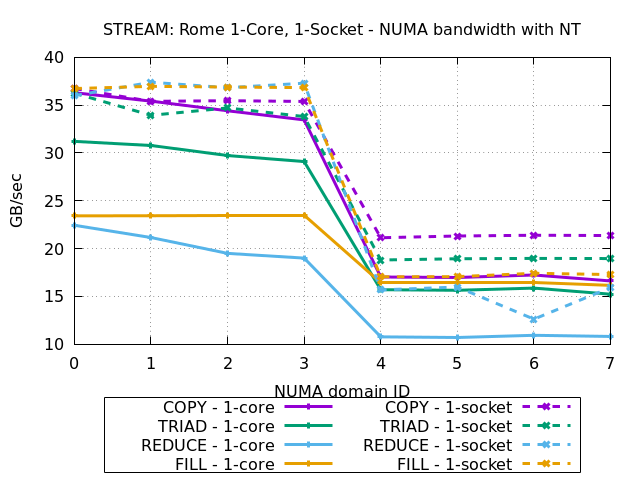
\includegraphics[width=0.3\textwidth]{../mem_bw_numa/Rome_numa_nps4_compact_nt}
    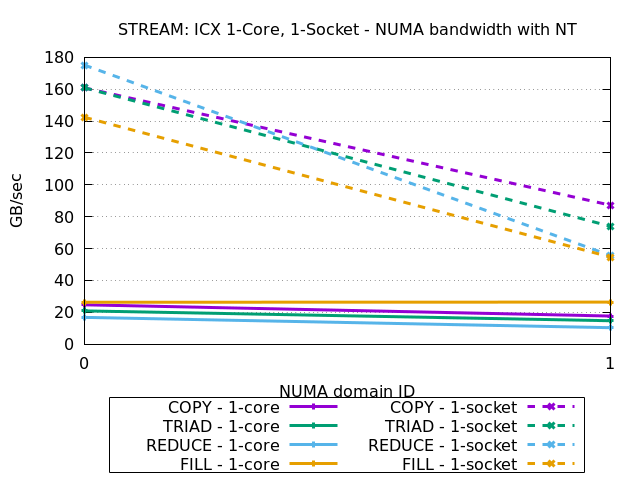
\includegraphics[width=0.3\textwidth]{../mem_bw_numa/ICX_numa_nps1_compact_nt}
    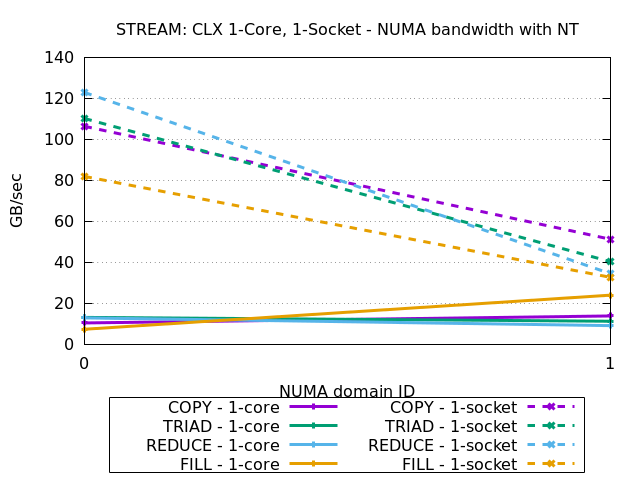
\includegraphics[width=0.3\textwidth]{../mem_bw_numa/CLX_numa_nps1_compact_nt}
    \caption{STREAM 1-Core, 1-socket NUMA bandwidth with NT}
    \label{figure:mem_bw_numa_nt}
\end{figure}



\subsection{Sub-NUMA Clustering}
CLX supports SNC-2, whereas ICX supports SNC-2, 4. To be filled when performance data with SNC-2, SNC-4.





\end{document}




















\begin{comment}

\begin{table}[h!]
\centering
\begin{tabular}{|c|c|c|}  \hline
Kernel & Rome/ICX RFO & Rome/ICX NT \\ \hline
Copy & 1.51x & 3.84x \\ \hline
Triad & 1.73x & 2.69x \\ \hline
Reduce & 2.26x & 2.24x \\ \hline
Fill & 1.97x & 1.53x \\ \hline
\end{tabular}
\caption{1-core peak bandwdith: Rome, ICX}
\label{table:mem_bw_core_rome_icx}
\end{table}

\begin{table}[h!]
\centering
\begin{tabular}{|c|c|c|}  \hline
Kernel & ICX/CLX RFO & ICX/CLX NT \\ \hline
Copy & 0.99x & 0.90x \\ \hline
Triad & 0.99x & 0.74x \\ \hline
Reduce & 0.73x & 0.77x \\ \hline
Fill & 0.66x & 2.11x \\ \hline
\end{tabular}
\caption{1-core peak bandwdith: ICX, CLX}
\label{table:mem_bw_core_icx_clx}
\end{table}

\begin{table}[h!]
\centering
\begin{tabular}{|c|c|c|} \hline
Kernel & ICX/Rome RFO & ICX/Rome NT \\ \hline
Copy & 1.40x & 0.99x \\ \hline
Triad & 1.36x & 1.27x \\ \hline
Reduce & 1.31x & 0.99x \\ \hline
Fill & 1.76x & 0.89x \\ \hline
\end{tabular}
\caption{1-socket peak bandwdith: RFO}
\label{table:mem_bw_socket_rome_icx}
\end{table}

\begin{table}[h!]
\centering
\begin{tabular}{|c|c|c|}  \hline
Kernel & ICX/CLX RFO & ICX/CLX NT \\ \hline
Copy & 2.03x & 1.45x \\ \hline
Triad & 1.87x & 1.44x \\ \hline
Reduce & 1.40x & 1.39x \\ \hline
Fill & 2.82x & 1.71x \\ \hline
\end{tabular}
\caption{1-socket peak bandwdith: ICX, CLX}
\label{table:mem_bw_socket_icx_clx}
\end{table}


\appendix
\appendixpage
\addappheadtotoc
\section{1-socket RFO vs NT Stores Scaling}

\begin{figure}[!hb]
    \centering
    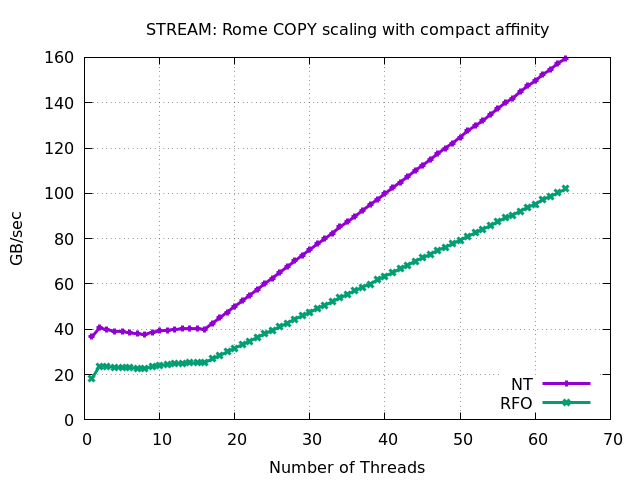
\includegraphics[width=0.45\textwidth]{../mem_bw_scale/Rome_scale_compact_Copy_nt_rfo}
    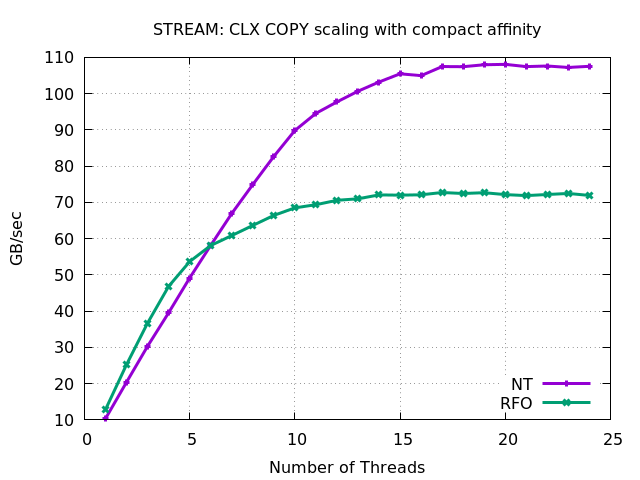
\includegraphics[width=0.45\textwidth]{../mem_bw_scale/CLX_scale_compact_Copy_nt_rfo}
    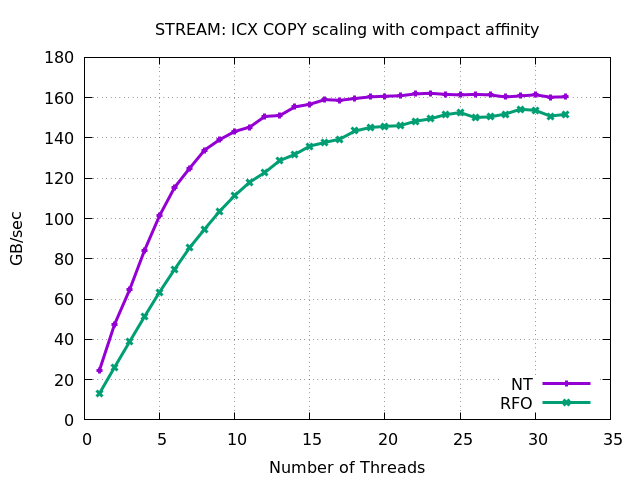
\includegraphics[width=0.45\textwidth]{../mem_bw_scale/ICX_scale_compact_Copy_nt_rfo}
    \caption{STREAM 1-socket DRAM bandwidth Scaling: RFO vs NT for Copy}
    \label{figure:mem_bw_scale_compact_copy_nt_rfo}
\end{figure}

\begin{figure}[!hb]
    \centering
    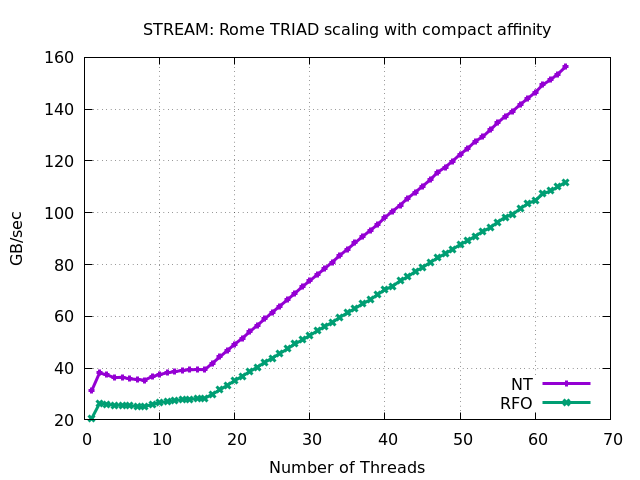
\includegraphics[width=0.45\textwidth]{../mem_bw_scale/Rome_scale_compact_Triad_nt_rfo}
    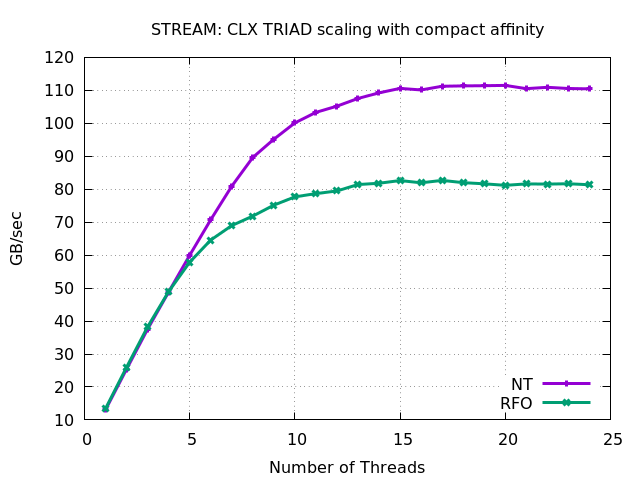
\includegraphics[width=0.45\textwidth]{../mem_bw_scale/CLX_scale_compact_Triad_nt_rfo}
    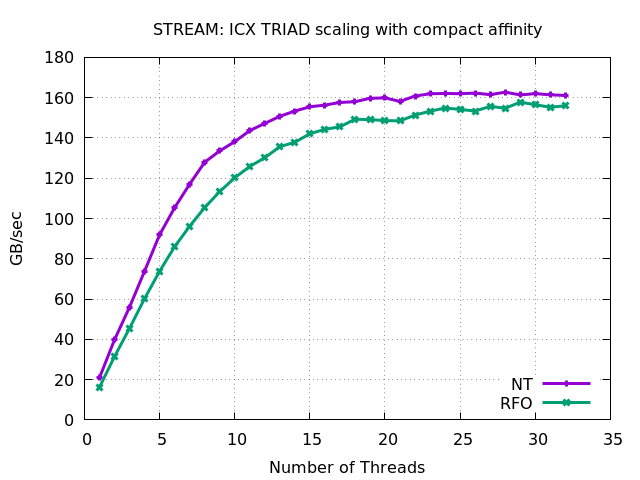
\includegraphics[width=0.45\textwidth]{../mem_bw_scale/ICX_scale_compact_Triad_nt_rfo}
    \caption{STREAM 1-socket DRAM bandwidth Scaling: RFO vs NT for Triad}
    \label{figure:mem_bw_scale_compact_triad_nt_rfo}
\end{figure}

\begin{figure}[!hb]
    \centering
    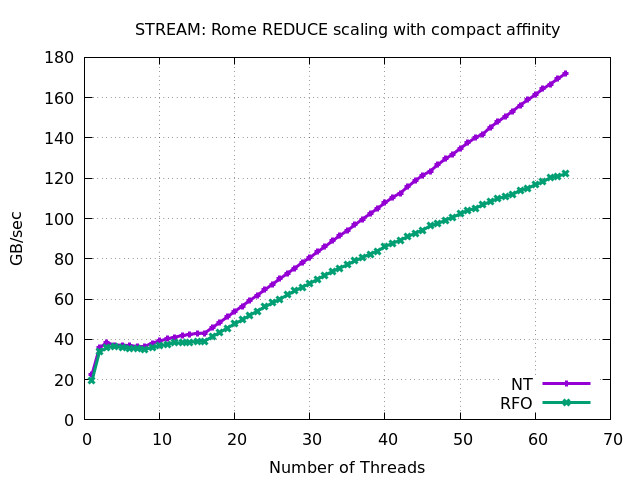
\includegraphics[width=0.45\textwidth]{../mem_bw_scale/Rome_scale_compact_Reduce_nt_rfo}
    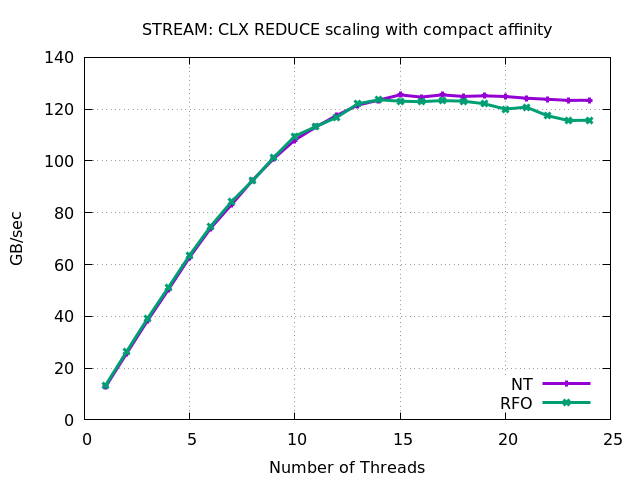
\includegraphics[width=0.45\textwidth]{../mem_bw_scale/CLX_scale_compact_Reduce_nt_rfo}
    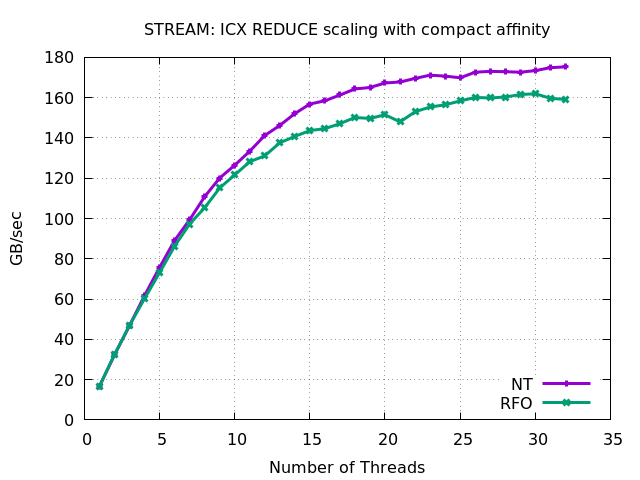
\includegraphics[width=0.45\textwidth]{../mem_bw_scale/ICX_scale_compact_Reduce_nt_rfo}
    \caption{STREAM 1-socket DRAM bandwidth Scaling: RFO vs NT for Reduce}
    \label{figure:mem_bw_scale_compact_reduce_nt_rfo}
\end{figure}

\begin{figure}[!hb]
    \centering
    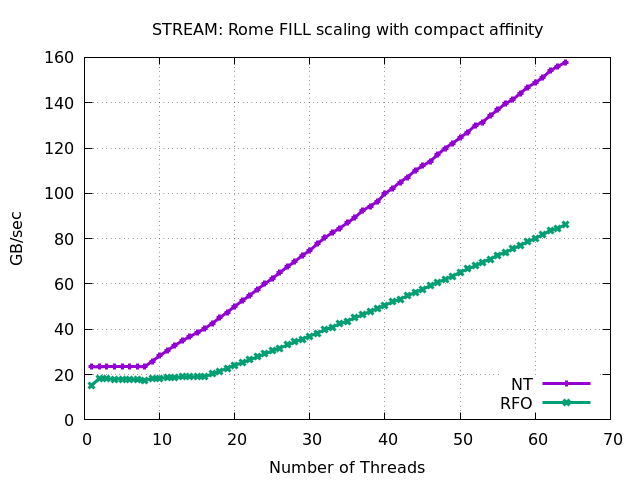
\includegraphics[width=0.45\textwidth]{../mem_bw_scale/Rome_scale_compact_Fill_nt_rfo}
    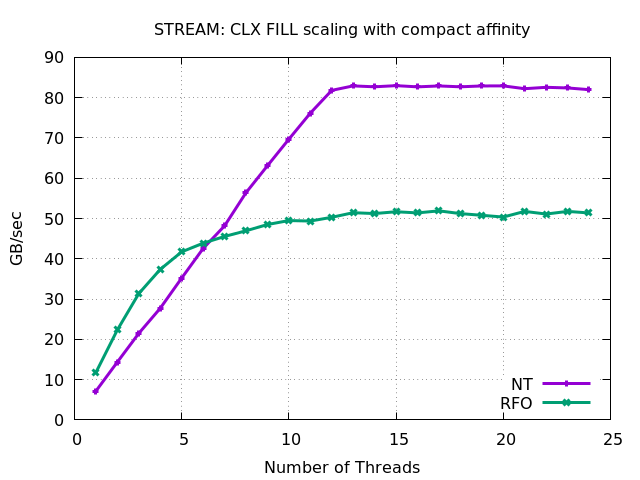
\includegraphics[width=0.45\textwidth]{../mem_bw_scale/CLX_scale_compact_Fill_nt_rfo}
    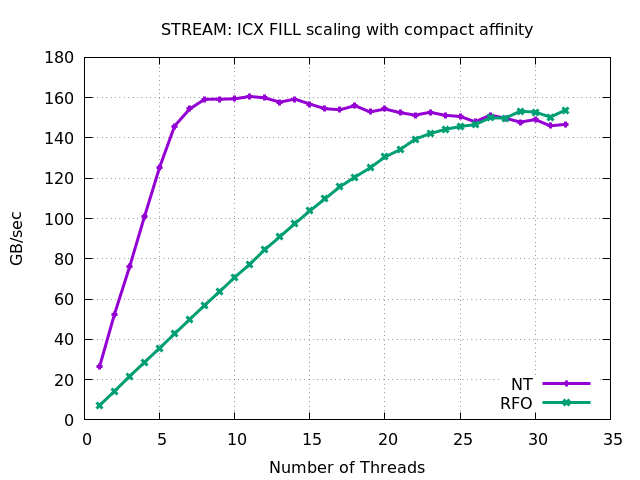
\includegraphics[width=0.45\textwidth]{../mem_bw_scale/ICX_scale_compact_Fill_nt_rfo}
    \caption{STREAM 1-socket DRAM bandwidth Scaling: RFO vs NT for Fill}
    \label{figure:mem_bw_scale_compact_fill_nt_rfo}
\end{figure}






\end{comment}

